% fig-iii-20.tex — III.20: inscribed angle theorem.
\begin{figure}[H]
\centering
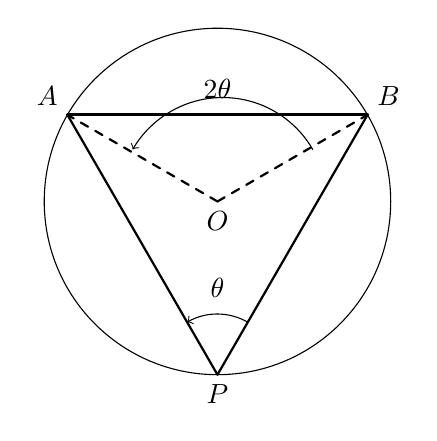
\begin{tikzpicture}[scale=1.1, line cap=round]
  \coordinate (O) at (0, 0);
  \def\r{2}
  \draw[thin] (O) circle (\r);
  \coordinate (A) at ({\r*cos(150)}, {\r*sin(150)}); % on circle, left
  \coordinate (B) at ({\r*cos(30)},  {\r*sin(30)});  % on circle, right
  \coordinate (P) at ({\r*cos(270)}, {\r*sin(270)}); % on circle, bottom (point opposite arc)
  % Chord AB.
  \draw[very thick] (A) -- (B);
  % Inscribed angle from P.
  \draw[thick] (P) -- (A);
  \draw[thick] (P) -- (B);
  % Central angle from O.
  \draw[thick, dashed] (O) -- (A);
  \draw[thick, dashed] (O) -- (B);
  \node[below] at (O) {$O$};
  \node[above left]  at (A) {$A$};
  \node[above right] at (B) {$B$};
  \node[below] at (P) {$P$};
  % Indicate angles.
  \draw[->, thin] (1.1, 0.6) arc[start angle=30, end angle=150, radius=1.2];
  \node at (0, 1.3) {$2\theta$};
  \draw[->, thin] (P) ++(60:0.7) arc[start angle=60, end angle=120, radius=0.7];
  \node at (0, -1.0) {$\theta$};
\end{tikzpicture}
\caption{Proposition III.20. The central angle $\angle AOB$ is twice
the inscribed angle $\angle APB$ subtending the same arc $AB$.
Corollary: all inscribed angles on the same arc are equal.}
\label{fig:III.20}
\end{figure}
